% Appendix A

\chapter{Search Algorithms} % Main appendix title

\label{AppendixB} % For referencing this appendix elsewhere, use 

In this appendix, the search algorithms used for this project are explained in more detail and how they have been adapted for this particular application.\\\\
These two search algorithms are used to find a target value in a sorted list of values. For this project, what we are trying to find is the minimum value for the cost function, and the list of values are all the integers between the minimum possible value for the cost function and the maximum possible value for it.

\begin{center}
	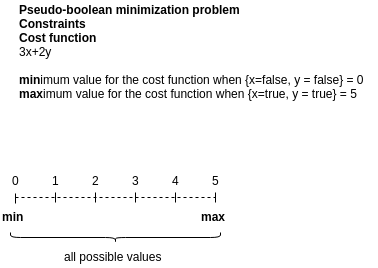
\includegraphics[width=0.8\textwidth]{Figures/Search_space.png}
	\captionof{figure}{Search Space}
	\label{search_space}
\end{center}
As the reader can see from the figure above, the search problem we are facing can be described as one where the search space is formed by integers between \emph{min} and \emph{max} and our target value is unknown.

\paragraph{How can we know that a value is the minimum, i.e. our target?\\}
If $m$ is the minimum value, we know that the constraint formed by $cost function \leq m$ is satisfiable whereas the constraint $cost function \leq m-1$ is unsatisfiable.\\\\
This is the property used to check if the value found is minimum or not.

\section{Linear search}

Linear search is an algorithm which sequentially checks all the values for the target value until it is found or all the elements have been visited.\\
The search can start with the smallest value or the biggest one. For this application, the initial value is \emph{max} and the algorithm traverse the search space descending until \emph{min}.\\
This decision was made because proving satisfiability of a problem is easier (faster) than proving it is unsatisfiable. Also, given $m$ and $n$ where $n < m$, if $cost function \leq m$ is unsatisfiable then $cost function \leq n$ will also be unsatisfiable. \\
As previously said, the algorithm starts with \emph{max}, which means that it generates the Pseudo-Boolean constraint $cost function \leq max$. If the problem is unsatisfiable with this value, it can be deduced that with other values will also be unsatisfiable and therefore the search can end.\\
Otherwise, it keeps this value as the possible minimum and tries the next one until it finds an unsatisfiable one or the \emph{min}, which is the last value to be checked.\\
Once the algorithm finished, the last found possible value becomes the minimum, or if no possible minimum was found, the problem is unsatisfiable.

\section{Binary search}
Binary search is an algorithm which looks for a value in a given sorted input.\\
As before, our inputs is the integers between \emph{min} and \emph{max}, and therefore they are sorted.\\
In the beginning, Binary search takes the middle value and compares it with the target value. If it is bigger than the target, then it looks for the value in the subspace between minimum value and the value before the middle one. If it is smaller than the target, then it looks for the value in the subspace between the value after the middle one and the maximum.\\
For this application, the leftmost value of the search is \emph{min}, and the rightmost value for the search is \emph{max}. Again, our target value is the minimum one. For each iteration, the algorithm checks that the left side of the problem is less or equal than the right side because otherwise, the state of the search would be incorrect. \\
If this is true, then it gets the middle value between them and generates the constraint $cost function \leq middle value$, which is added with the other constraints and then encoded into a CNF. If the CNF is satisfiable, then the middle value is stored as a possible minimum, and the search continues with a new space contained between the left side and the integer between the middle value. Otherwise, if the CNF is unsatisfiable, it checks if the stored possible minimum is exactly the integer after the middle value because then the integer would be the minimum value.\\
If not, it continues the search with a new space contained between the integer after the middle value and the right side.